\section{Software Architecture}
This section serves as a guide to the high level structure of the application. It defines the key components as well as their relationship with each other.
Moreover, it describes the fundamental design patterns and architecture that define the application and its functionalities. 
The diagram presented below helps to gain better understanding of the application's architecture.
\begin{figure}[H]
    \centering
    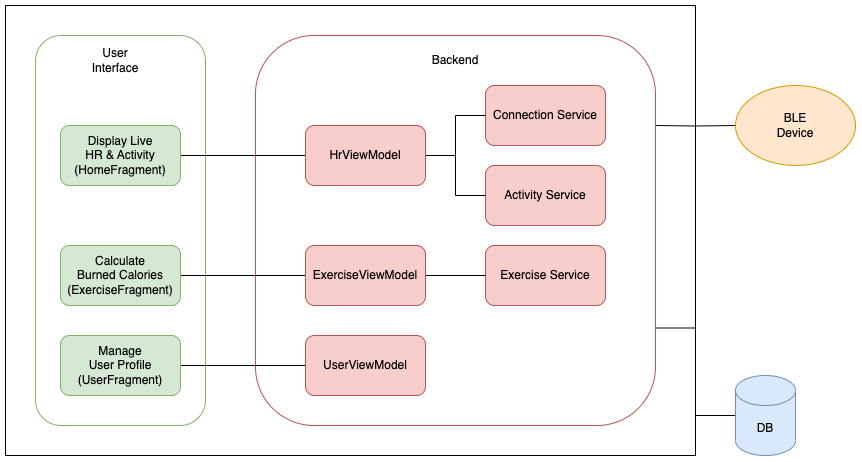
\includegraphics[width=1\textwidth]{diagrams/architecture-diagram.drawio.png}
    \caption{Software architecture diagram}
    \label{fig:soft_diagram}
\end{figure}
The project follows the Model-View-ViewModel (MVVM) architectural pattern. The user interface, which is responsible for displaying the features to the user, represents the View. 
The Model is represented by the data and the business logic of the application, for instance, the entities and the functionalities such as live heart rate monitor, activity monitoring, exercise service, and user data management. 
The ViewModels facilitate the communications between the models and the views through which the views can access and interact with the data and operations of the models.

The user interface consists of three main components which extends Fragment\footnote{Based on The Official Android Documentation, a Fragment represents a reusable portion of your app's UI. A fragment defines and manages its own layout, has its own lifecycle, and can handle its own input events. \autocite{android-fragments}}. 
The HomeFragment displays real-time heart rate data and the activity monitor. It serves as the initial entry point for the users as they log in to the application. As it shows live heart rate data and activity, it holds a connection to the HrViewModel.
The ExerciseFragment presents the number of calories burned in an exercise based on the user's heart rate. It maintains a connection with the ExerciseViewModel. Lastly, the UserFragment, which is connected to the UserViewModel, displays the user's data and provide the necessary UI components to support data management.

The backend is in charge of the core functionalities of the application, which involve establishing a connection to the database.
As one of the core components, the connection service maintains the connection between the BLE device and the application. It actively listens to the heart rate data being broadcasted by the BLE device. 
The activity service determines the current activity status based on the user's heart rate and age. 
On the other hand, the exercise service tracks the user's energy expenditure during training based on the user's heart rate and physical measurements such as weight, age, and gender. Both the exercise service and activity service subscribe to an event, where the heart rate data is published by the connection service. This enables the services to receive the heart rate data seamlessly and process it accordingly.
Lastly, the UserViewModel is responsible for the management of the user's data and facilitates CRUD operations related to the user's data.
